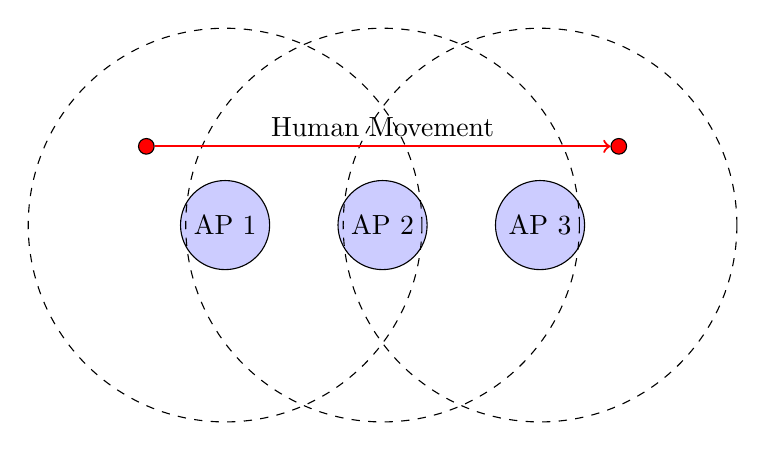
\begin{tikzpicture}
% Access Points
\node[draw, circle, fill=blue!20, minimum size=1cm] (ap1) at (0,0) {AP 1};
\node[draw, circle, fill=blue!20, minimum size=1cm] (ap2) at (2,0) {AP 2};
\node[draw, circle, fill=blue!20, minimum size=1cm] (ap3) at (4,0) {AP 3};

% Ranges
\draw[dashed] (ap1) circle (2.5cm);
\draw[dashed] (ap2) circle (2.5cm);
\draw[dashed] (ap3) circle (2.5cm);

% Person's movement
\node[draw, circle, fill=red, inner sep=2pt] (start) at (-1,1) {};
\node[draw, circle, fill=red, inner sep=2pt] (end) at (5,1) {};
\draw[->, thick, red] (start) -- (end) node[midway, above, black] {Human Movement};
\end{tikzpicture}